\documentclass[12pt,a4paper]{article}
\usepackage{header}

\usepackage[bf,sf]{titlesec}
\usepackage[font={footnotesize,sf}]{caption}

\usepackage[colorlinks=true]{hyperref}

\usepackage{siunitx}
\sisetup{allow-number-unit-breaks, prefixes-as-symbols=false, output-decimal-marker={,}, list-final-separator={and}, range-phrase={--}, range-units=brackets}

\title{\textsf{\textbf{Pràctica 2: Oscil·lacions}}}
\author{Arnau Mas}
\date{9 de Gener 2018}

\begin{document}
\maketitle
\selectlanguage{catalan}

\begin{abstract}
	L'objectiu d'aquesta pràctica és estudiar la mecànica de l'oscil·lador amortit i forçat. El sistema que s'observarà consisteix d'una massa subjectada a dues molles. La posició de la massa es mesurarà amb un sensor de posició, així com la posició del motor que es farà servir per a excitar el sistema.

	En el cas de l'oscil·lador amortit, s'ha pogut observar la caiguda exponencial de l'amplitud amb el temps. Amb les mesures preses s'ha pogut calcular el coeficient de fregament, tot i que el valor obtingut discrepa considerablement amb el valor teòric. Pel cas forçat s'ha pogut observar el fenomen de ressonància, tant en termes d'amplitud com de desfasament. 
\end{abstract}

\section{Introducció i Objectius}\label{sec:intro}
L'objectiu d'aquesta pràctica és estudiar les característiques de l'oscil·lador amortit i forçat. Més concretament, en el cas de l'oscil·lador amortit es comprovarà l'efecte del fregament sobre la freqüència d'oscil·lació, així com la caiguda exponencial de l'amplitud amb el temps. Pel que fa al cas de l'oscil·lador forçat, es verificarà l'impacte que té la freqüència forçada sobre l'amplitud i el desfasament.

La dinàmica de l'oscil·lador harmònic simple està governada per la següent equació diferencial:
\begin{equation}
 	m\ddot{x} = -kx, \label{eq:oscilador harmonic simple}
\end{equation}
on \( m \) és la massa de la partícula, \( k \) és la constant elàstica de l'oscil·lador i \( x \) és la posició de la partícula, prenent com a origen el punt d'equilibri de l'oscil·lador. Aquesta equació és conseqüència immediata d'aplicar la segona llei de Newton considerant que sobre la partícula només hi actua una força atractiva proporcional a la distància entre la partícula i un punt d'equilibri; és a dir, una força de la forma \( F = -kx \). 

Tradicionalment es defineix la quantitat \( \omega_0 = \sqrt{k / m} \), anomenada freqüència pròpia del sistema. El nom té sentit ja que les solucions de l'equació \ref{eq:oscilador harmonic simple} són trajectòries de la forma
\begin{equation}
  x(t) = A_1\cos{\omega_0 t} + A_2\sin{\omega_0 t}; \label{eq:solucions mhs 1}
\end{equation}
és a dir, oscil·lacions periòdiques de freqüència \( \omega_0 \). Els paràmetres \( A_1 \) i \( A_2 \) depenen de les condicions inicials. Podem reescriure \ref{eq:solucions mhs 1} com
\begin{equation}
  x(t) = A\cos({\omega_0 t + \phi}), \label{eq:solucions mhs 2}
\end{equation}
de manera que aquests nous paràmetres tenen un significat físic més evident: \( A \) és l'amplitud del moviment i \( \phi \) n'és la fase.

La dinàmica de l'oscil·lador amortit apareix quan afegim un terme que depèn de la velocitat a l'equació del moviment harmònic simple. Aquest terme, que correspon a una força de la forma \( F = -b\dot{x} \), s'interpreta com un terme de fregament. Per a escriure l'equació és convenient introduir el factor \( \beta = b/2m \), que anomenem coeficient de fregament. Així, fent servir les definicions anteriors, l'equació que governa l'oscil·lador harmònic amortit és
\begin{equation}
  \ddot{x} + 2\beta \dot{x} + \omega_0^2 x = 0. \label{eq:oscilador harmonic amortit}
\end{equation}

Per a condicions d'infraamortiment, és a dir, quan \( \beta < \omega_0 \), es pot comprovar que les solucions són trajectòries de la forma
\begin{equation}
  x(t) = Ae^{-\beta t}\cos({\omega t + \phi}) \label{eq:solucions mha}
\end{equation}
on \( A \) i \( \phi \) són, igual com abans, l'amplitud màxima i la fase inicial, respectivament. La freqüència \( \omega \) és la nova freqüència d'oscil·lació i ve donada per la relació
\begin{equation}
  \omega^2 = \omega_0^2 - \beta^2. \label{eq:nova frequencia}
\end{equation}
Ara és clar perquè aquesta classe de moviments només té sentit en condicions d'infraamortiment. Cal remarcar que, tot i que l'amplitud decaigui amb el temps, la freqüència d'oscil·lació, i per tant el període, es manté constant. 

El cas de l'oscil·lador forçat és, en termes matemàtics, la versió no homogènia de l'oscil·lador amortit. L'equació diferencial corresponent és 
\begin{equation}
  \ddot{x} + 2\beta\dot{x} + \omega_0^2x = \dfrac{F(t)}{m}. \label{eq:oscilador harmonic forçat}
\end{equation}
El terme \( F(t) \) correspon a la força que s'aplica sobre el sistema. En el cas de la pràctica, es considerarà una força sinusoidal de la forma \( F(t) = F_0 \cos{\omega_f t} \). La freqüència \( \omega_f \) l'anomenarem freqüència forçada. 

En condicions d'infraamortiment, el moviment de l'oscil·lador harmònic forçat és
\begin{equation}
 	x(t) = Ae^{-\beta t}\cos({\omega t + \phi}) + \dfrac{F_0}{md}\cos({\omega_f t - \theta}). \label{eq:solucions mhf}	
\end{equation}
El primer terme s'anomena el terme transitori. Veiem que decau exponencialment amb el temps, així que per a valors de temps prou grans és negligible. En aquestes condicions diem que l'oscil·lador està en el règim estacionari. Les quantitats \( d \) i \( \theta \) depenen de \( \omega_0 \), \( \beta \) i \( \omega_f \). Quan \( \omega_f = \omega_0 \) el sistema oscil·la amb la màxima energia possible i diem que està en ressonància. En aquestes circumstàncies, la diferència de fase entre la força externa ---és a dir, el motor--- i l'oscil·lador és de \( \pi/2 \) radiants. Per valors de freqüència forçada inferiors a \( \omega_0 \), la diferència de fase és propera a 0, mentre que per a valors prous superiors a \( \omega_0 \) s'acosta a \( \pi \) radiants. El màxim d'amplitud no es dóna quan \( \omega_f = \omega_0 \), ara bé, per \( \beta \) prou petit, el pic d'amplitud succeeix per a un valor de \( \omega_f \) proper a \( \omega_0 \).  

\section{Materials i Mètodes}\label{sec:metodes}
\subsection{Oscil·lador amortit}
El muntatge experimental consisteix en una lliscadora de massa \data{348,6}{0,1}{g} lligat a dues molles de constants \( k_1 = \data{3,8}{0,1}{N.m^{-1}} \) i \( k_2 = \data{3,7}{0,1}{N.m^{-1}} \). Com que les molles actuen en paral·lel, és equivalent considerar un sistema format per una única molla de constant \( k = k_1 + k_2 = \data{7,6}{0,2}{N.m^{-1}} \).

El sistema està muntat al damunt d'una via d'aire comprimit, de manera que els efectes del fregament amb la via quedin minimitzats. D'aquesta manera, el sistema està basicament sotmès al fregament de l'aire, garantint condicions d'infraamortiment. Efectivament, quan el sistema es desplaça de la posició d'equilibri es poden observar oscil·lacions. Per a fer les medicions, un cop el sistema comença a oscil·lar, s'activa la recollida de dades del sensor de posició colocat també sobre la via d'aire. Aquest sensor mesura la posició del sistema amb l'origen fixat en la posició del propi sensor. Així doncs, si volem tenir dades d'amplitud en la referència estàndard ---amb l'origen en la posició d'equilibri de les molles---, cal considerar la posició del punt d'equilibri relativa a la posició del sensor.

El sistema es deixa oscil·lar temps suficient fins que l'amplitud de les oscil·lacions sigui gairebé nul·la. Amb el programa DataStudio s'obté una visualització de les dades. En primer lloc, per a determinar la freqüència d'oscil·lació \( \omega \) es fa servir el fet que, en el moviment harmònic amortit, el període d'oscil·lació és constant. El període és una quantitat mesurable, i fent servir la relació \( \omega = 2\pi/T \), es pot obtenir el valor de \( \omega \). Per a minimitzar la incertesa en el període, es mesura primer el temps, \( T_N \), que triga el sistema en fer \( N \) oscil·lacions i després es calcula el període com \( T = T_N / N \). Així, si la incertesa en la mesura de \( T_N \) és \( u(T_N) \), la incertesa del període és \( u(T) = u(T_N)/N \).

Pel que fa a l'anàlisi de l'amplitud, es recull el valor de l'amplitud corresponent a cada cicle mitjançant la visualització de DataStudio per realitzar l'ajust lineal. Tot i que la precisió del sensor de posició és de \SI{1}{mm}, cal remarcar que la incertesa que considerem per a les mesures d'amplitud no pot ser tant baixa. Això és perquè la mesura d'amplitud s'hauria de fer en el moment exacte en que el sistema té velocitat nul·la. Com que el sensor pren mesures a intervals de temps comparables amb el període d'oscil·lació, la mesura de posició de valor més gran de cada cicle es fa lleugerament abans o després de l'instant de màxim desplaçament.

Amb les dades d'amplitud i els temps corresponents recollits, es procedeix a fer l'ajust lineal. Aquest ajust es fa entre el logaritme (natural) de l'amplitud i el temps. Si és un bon ajust, podem concloure que la relació entre l'amplitud i el temps és exponencial, tal i com prediu la teoria. Més en detall tenim que la predicció teòrica és 
\begin{equation}
  A(t) = Ae^{-\beta t},
\end{equation}
per l'equació \ref{eq:solucions mha}. Si podem fer un ajust lineal significatiu entre \( \log{A} \) i \( t \) tenim que hi ha una relació de la forma
\begin{equation}
  \log{A(t)} = \lambda t + \alpha
\end{equation}
i per tant 
\begin{equation}
  A(t) = e^{\alpha}e^{\lambda t}.
\end{equation}
Si l'ajust és bo, concloem que els resultats estan d'acord amb la teoria. A més haurem trobat el valor del coeficient d'amortiment \( \beta \), ja que \( -\lambda = \beta \).

Finalment, coneguts \( \beta \) i \( \omega_0 \) calcularem \( \sqrt{\omega_0^2 - \beta^2} \) i el compararem amb el valor mesurat de la freqüència, per verificar l'equació \ref{eq:nova frequencia}.

\subsection{Oscil·lador forçat}
El muntatge de la segona part és idèntic a la primera però afegint un motor a l'extrem de les molles i un sensor adicional per mesurar-ne la posició. Per a pendre les mesures s'activa el motor i s'espera a que el sistema estigui en el règim estacionari. Aleshores es mesuren simultàniament les posicions del motor i de la massa. Aquest procés es repeteix per a diferents valors de la freqüència forçada: alguns per sota de la freqüència pròpia i alguns per sobre. El motor utilitzat permet modular-ne la freqüència. Ara bé, es van fer unes mesures preliminars comparant la freqüència llegida al propi motor amb el valor obtingut fent una mesura directa i es va trobar que el valor que donava el motor introduïa un error relatiu d'aproximadament un \( 9\% \) respecte el valor real. Per aquest motiu, per determinar la freqüència forçada vam fer sempre una mesura directa.

Per mesurar l'amplitud del moviment es procedeix com abans. Com que ara l'amplitud és constant, es prenen mesures d'aquesta en diferents màxims i es pren la mitjana.

Per a trobar el desfasament entre el motor i la massa, \( \theta \), es mesura la diferència de temps, \( \Delta t \), entre un màxim en la posició de la massa i el màxim corresponent en el motor i es fa servir que
\begin{equation}
  \theta = 2\pi \dfrac{\Delta t}{T}, 
\end{equation}
on \( T \) és el període de l'oscil·lació ---és el mateix per a la massa que per al motor---, que es mesura igual com en el cas amortit.  

\section{Resultats} \label{sec:resultats}
\subsection{Oscil·lador amortit}
En primer lloc es van pendre mesures per determinar els paràmetres del sistema. La freqüència pròpia del sistema és \( \omega_0 = \data{4,66}{0,05}{rad.s^{-1}} \). El període d'oscil·lació del sistema en les condicions de l'experiment és \( T = \data{1,414}{0,007}{s} \) i per tant amb una freqüència de \( \omega = \data{4,46}{0,03}{rad.s^{-1}} \). 

\begin{figure}[htb]
	\centering
	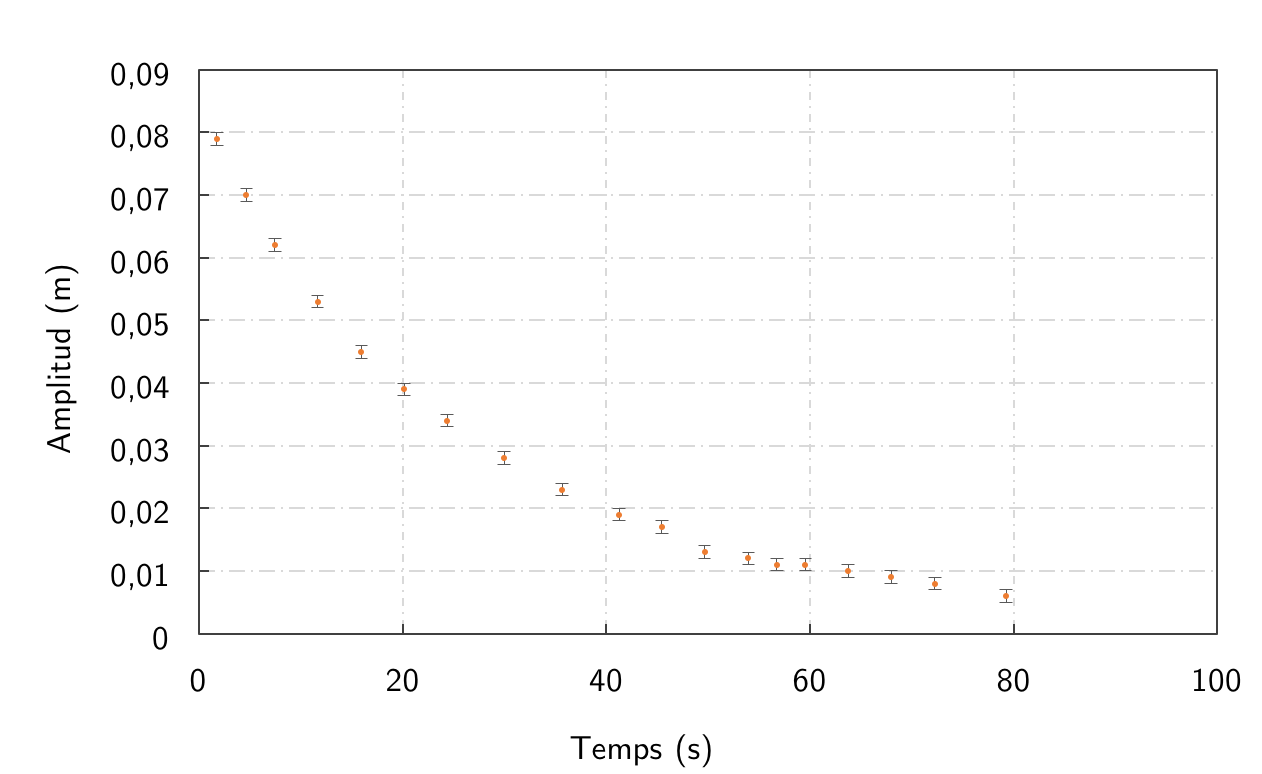
\includegraphics[scale=0.6]{amplitud.png}
	\caption{Amplitud màxima en funció del temps. Es pot apreciar molt clarament la caiguda exponencial de l'amplitud amb el temps.}
	\label{fig:amplitud en funcio del temps}
\end{figure}

\begin{figure}[htb]
  \centering
	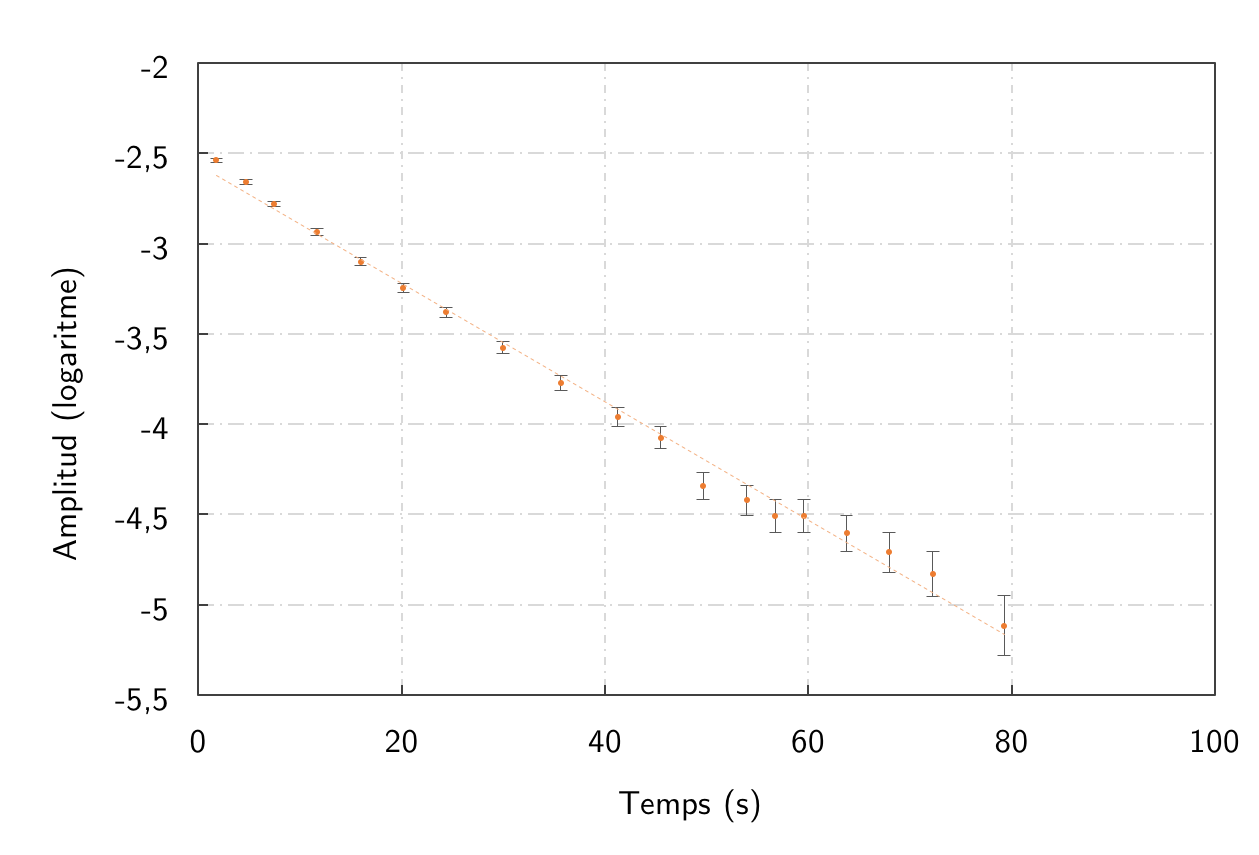
\includegraphics[scale=0.6]{log(A).png}
	\caption{Logaritme de l'amplitud en funció del temps. Es veu clarament que les dues magnituds estan relacionades linealment, la qual cosa es tradueix a una relació exponencial entre l'amplitud i el temps.}
	\label{fig:log(amplitud) en funcio del temps}
\end{figure}

La figura \ref{fig:amplitud en funcio del temps} mostra l'evolució amb el temps de l'amplitud de l'oscil·lació. A primera vista ja es veu que la caiguda és exponencial amb el temps. Per a fer una anàlisi més quantitativa, però, es va fer un ajust lineal entre el logaritme de l'amplitud i el temps, tal i com s'explica a la secció \ref{sec:metodes}. La figura \ref{fig:log(amplitud) en funcio del temps} mostra això.

La pendent de la recta de regressió obtinguda pel mètode de mínims quadrats és \data{-3,28}{0,06d-2}{s^{-1}}. Això ens dóna el valor del coeficient d'amortiment: \( \beta = \data{-3,28}{0,06d-2}{s^{-1}} \). Amb un coeficient \( R^2 \) de \num{0,993} podem afirmar que l'ajust és significatiu. L'ordenada a l'origen és \data{-2,57}{0,02}{}.

Fent servir l'equació \ref{eq:nova frequencia}, amb el valor de \( \beta \) determinat experimentalment, trobem que el valor de la nova freqüència hauria de ser \data{4,66}{0,05}{rad.s^{-1}}.

\subsection{Oscil·lador forçat}

\begin{figure}[htb]
  \centering
	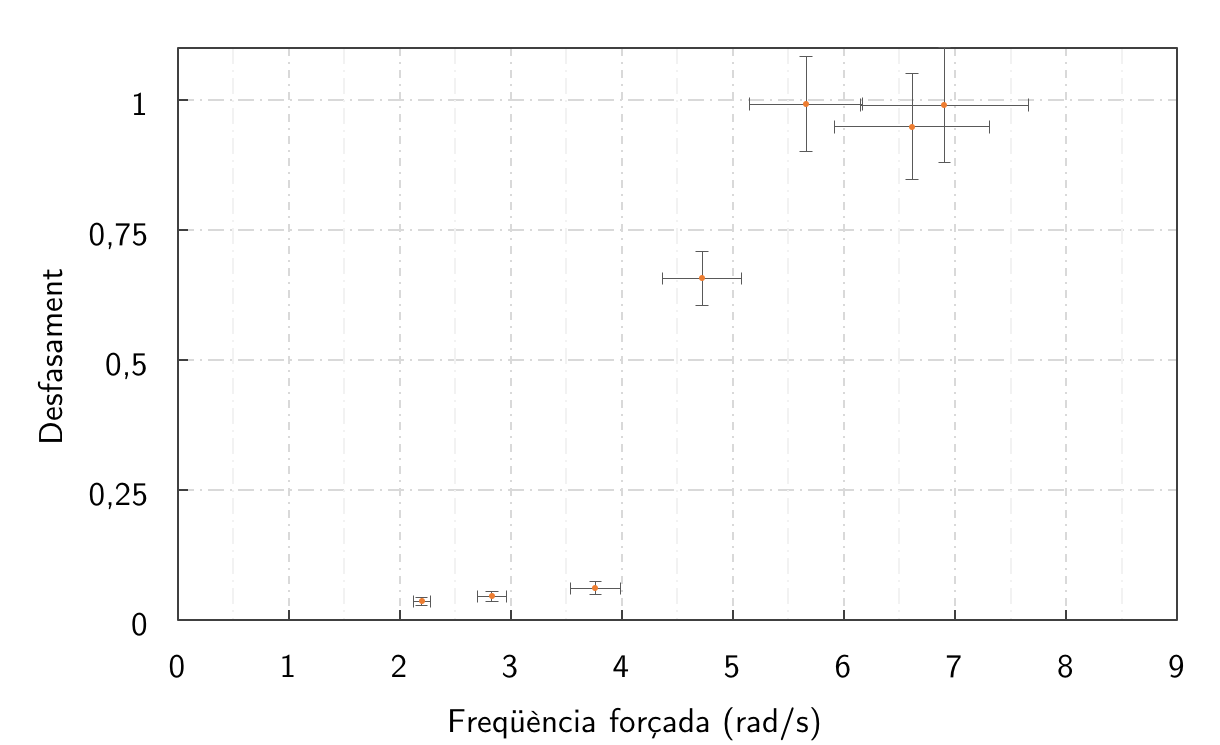
\includegraphics[scale=0.6]{desfasament.png}
	\caption{Desfasament entre el motor i l'oscil·lador en funció de la freqüència forçada. El desfasament és adimensional ja que està expresat com el quocient entre el desfasament en radiants i \SI{\pi}{rad}.}
	\label{fig:desfasament}
\end{figure}

\begin{figure}[htb]
  \centering
	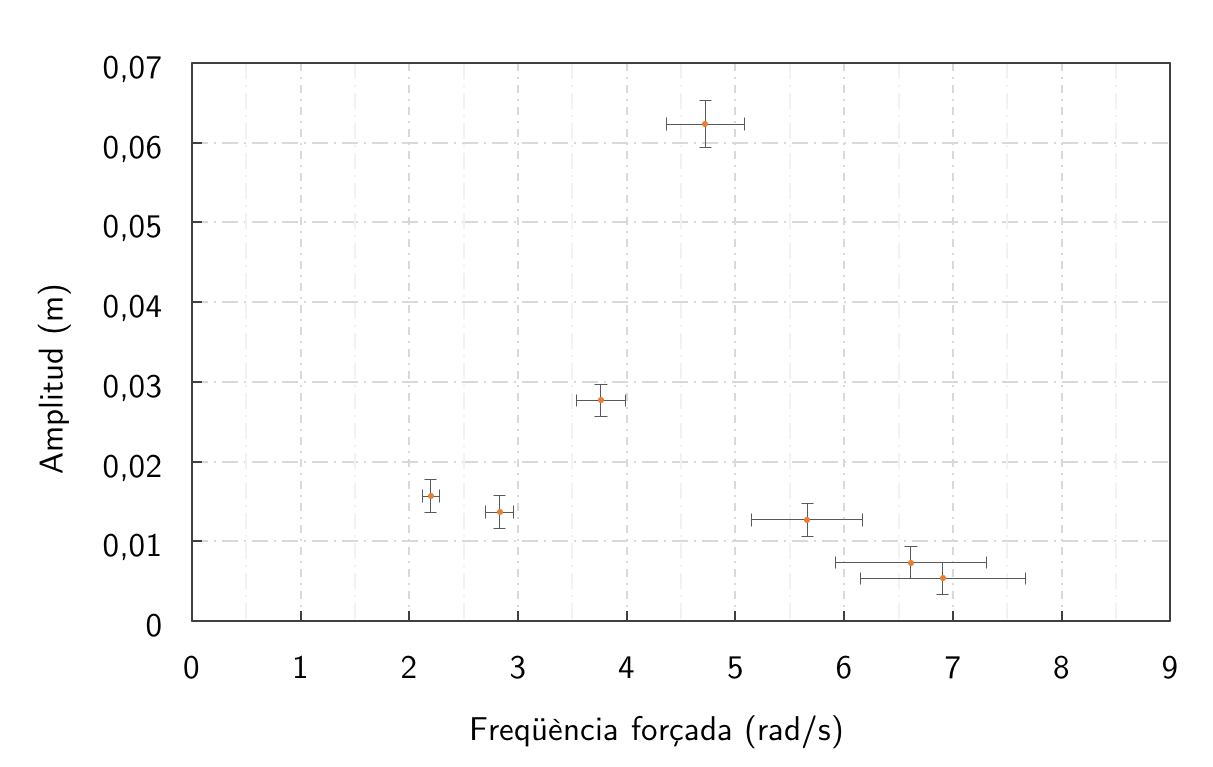
\includegraphics[scale=0.6]{ressonancia.png}
	\caption{Amplitud màxima d'oscil·lació en funció de la freqüència forçada.}
	\label{fig:amplitud en funcio de frequencia}
\end{figure}

Per aquesta secció es van realitzar mesures a sis freqüències diferents entre \data{2,20}{0,08}{rad.s^{-1}} i \data{6,9}{0,8}{rad.s^{-1}}. Seguint el mètode explicat a la secció \ref{sec:metodes}, es van determinar el desfasament i amplitud corresponents a cada freqüència.  

Pel que fa al desfasament es pot apreciar clarament com aquest és pràcticament nul per a freqüències inferiors a la freqüència pròpia, i gairebé 1 ---per tant \SI{\pi}{rad}--- per a freqüències superiors (figura \ref{fig:desfasament}).

A la figura \ref{fig:amplitud en funcio de frequencia} es pot apreciar com la variació de l'amplitud en funció de la freqüència forçada segueix el perfil característic d'un oscil·lador harmònic forçat, amb un pic al voltant de la freqüència pròpia.  

\section{Conclusions}\label{sec:conclusions}
Pel que fa a l'estudi de l'oscil·lador amortit, podem concloure, en base a la regressió lineal realitzada, que l'amplitud efectivament decau exponencialment amb el temps. En canvi, pel que fa a les freqüències, els dos valors obtinguts per \( \omega \) --- \data{4,46}{0,03}{rad.s^{-1}} experimentalment i \data{4,66}{0,05}{rad.s^{-1}} a partir de l'expressió \ref{eq:nova frequencia}--- són clarament no compatibles. La diferència entre el valor experimental i el valor teòric és de \SI{4,5}{\%}. Ara bé, si considerem el coeficient de fregament necessari perque la freqüència pròpia del sistema decaigués fins a la freqüència mesurada trobem que hauria de ser \data{1,4}{0,2}{s^{-1}}, molt allunyat del valor obtingut. Cal mencionar que el valor de \( \omega_0 \) es va determinar a partir d'una massa i constants elàstiques donades a priori i no mesurades. Així doncs és possible que la discrepància entre la freqüència teòrica i mesurada sigui deguda a un càlcul del valor teòric erroni a partir d'un valor de \( \omega_0 \) incorrecte.

Els resultats obtinguts en l'anàlisi de l'oscil·lador forçat són compatibles amb les prediccions de la teoria. Efectivament, veiem en la figura \ref{fig:desfasament} que per a valors de la freqüència per sota de \SI{4}{rad.s^{-1}}, el motor i el sistema oscil·len pràcticament en fase. I per a valors superiors a \SI{5}{rad.s^{-1}}, la diferència de fase és propera a 1. El canvi en el desfasament es produeix en l'interval \SIrange{4}{5}{rad.s^{-1}}, que és on es troba la freqüència fonamental del sistema. Per a un valor de freqüència de \data{4,7}{0,4}{rad.s^{-1}} el desfasament és lleugerament superior a \( \SI{\pi/2}{rad} \). Aquest desfasament és el desfasament més proper a \( \pi/2 \) que vam poder observar. Això sembla indicar, a més, que la freqüència pròpia del sistema és més propera a \SI{4,5}{rad.s^{-1}} que no al valor calculat inicialment, tal i com comentem abans. 

Finalment, tal i com s'aprecia a la figura \ref{fig:amplitud en funcio de frequencia}, el màxim d'amplitud degut a ressonància es produeix també en el rang \SIrange{4}{5}{rad.s^{-1}}, corroborant els resultats obtinguts en l'anàlisi del desfasament. Concloem, doncs, que l'oscil·lador forçat efectivament experimenta ressonància quan és excitat a la seva freqüència pròpia, i que això dóna lloc a una amplitud màxima i a una diferència de fase de \( \SI{\pi/2}{rad} \), tal i com prediu la teoria. 

\appendix
\section{Expressions per a les incerteses}
A continuació es donen les expressions utilitzades per al càlcul de les incerteses de les quantitats determinades en l'informe.

\begin{itemize}
	\item Freqüència natural, \( \omega_0 \):
		\begin{equation}
		 	u(\omega_0)^2 = \dfrac{1}{mk}u(k)^2 + \dfrac{\omega_0^2}{m^2}u(m)^2 
		\end{equation}
		
	\item Freqüència \( \omega \) (mesurada):
		\begin{equation}
		  u(\omega) = \dfrac{2\pi}{T^2}u(T)
		\end{equation}

	\item Freqüència \( \omega \) (calculada):
		\begin{equation}
		  u(\omega)^2 = \left(\dfrac{\omega_0}{\omega}u(\omega_0)\right)^2 + \left( \dfrac{\beta}{\omega} u(\beta) \right)^2
		\end{equation}
		
	\item Desfasament, \( \theta \):
		\begin{equation}
		  u(\theta)^2 = \left( \dfrac{\theta}{\Delta t} u(\Delta t) \right)^2 + \left( \dfrac{\theta}{T} u(T) \right)^2
		\end{equation}
		
		
\end{itemize}


\end{document}
